\section{General Overview}
\label{section:overview}
The model architecture of Llama 3 is illustrated in Figure~\ref{sph:fig:language_model_overview}.
The development of our Llama 3 language models comprises two main stages:

\begin{itemize}

\item \textbf{Language model pre-training.} We start by converting a large, multilingual text corpus to discrete tokens and pre-training a large language model (LLM) on the resulting data to perform next-token prediction. In the language model pre-training stage, the model learns the structure of language and obtains large amounts of knowledge about the world from the text it is ``reading’’. To do this effectively, pre-training is performed at massive scale: we pre-train a model with 405B parameters on 15.6T tokens using a context window of 8K tokens. This standard pre-training stage is followed by a continued pre-training stage that increases the supported context window to 128K tokens. See Section~\ref{section:pretraining} for details.

\item \textbf{Language model post-training.} The pre-trained language model has a rich understanding of language but it does not yet follow instructions or behave in the way we would expect an assistant to. We align the model with human feedback in several rounds, each of which involves supervised finetuning (SFT) on instruction tuning data and Direct Preference Optimization~\citep[DPO;][]{rafailov2024direct}. At this post-training\footnote{In this paper, we use the term ``post-training'' to refer to any model training that happens outside of pre-training.} stage, we also integrate new capabilities, such as tool-use, and observe strong improvements in other areas, such as coding and reasoning. See Section~\ref{section:finetuning} for details. Finally, safety mitigations are also incorporated into the model at the post-training stage, the details of which are described in Section~\ref{section:results_safety}. 

\end{itemize}

\begin{figure}[t]
    \centering
    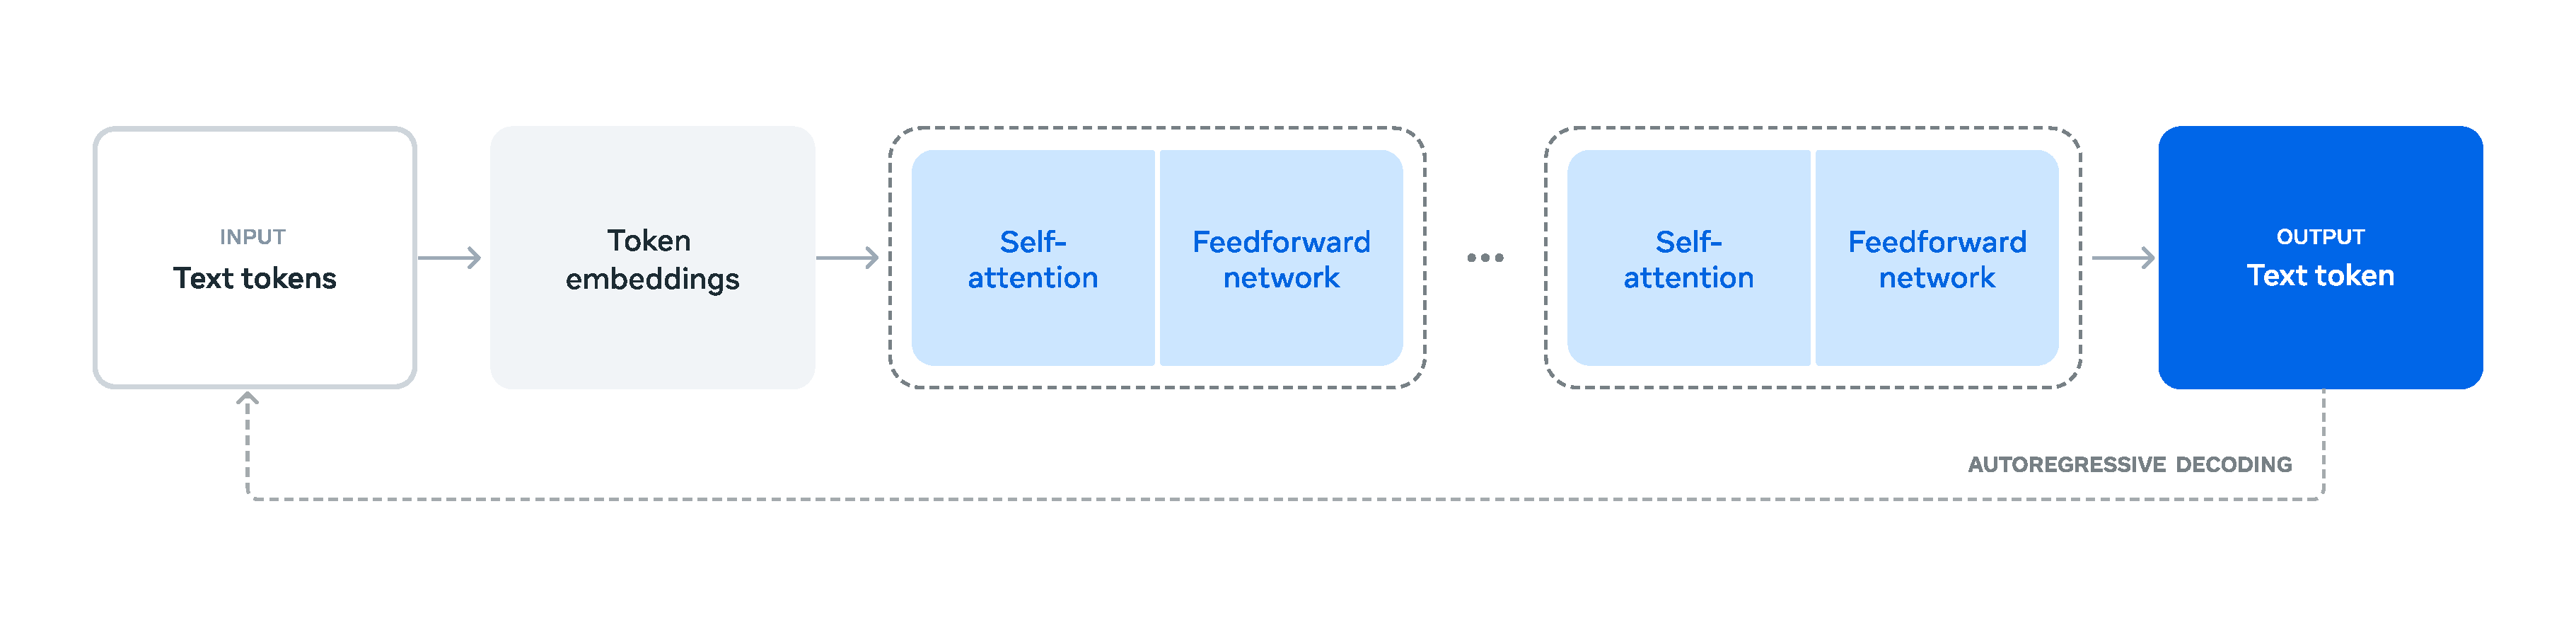
\includegraphics[width=\textwidth]{assets/llama3_language_architecture.pdf}
    \caption{\textbf{Illustration of the overall architecture and training of Llama 3.} Llama 3 is a Transformer language model trained to predict the next token of a textual sequence. See text for details.}
    \label{sph:fig:language_model_overview}
\end{figure}

The resulting models have a rich set of capabilities.
They can answer questions in at least eight languages, write high-quality code, solve complex reasoning problems, and use tools out-of-the-box or in a zero-shot way.

We also perform experiments in which we add image, video, and speech capabilities to Llama 3 using a compositional approach.
The approach we study comprises the three additional stages illustrated in Figure~\ref{sph:fig:multimodal_model_overview}:

\begin{itemize}

\item \textbf{Multi-modal encoder pre-training.} We train separate encoders for images and speech. We train our image encoder on large amounts of image-text pairs. This teaches the model the relation between visual content and the description of that content in natural language. Our speech encoder is trained using a self-supervised approach that masks out parts of the speech inputs and tries to reconstruct the masked out parts via a discrete-token representation. As a result, the model learns the structure of speech signals. See Section~\ref{section:vision} for details on the image encoder and Section~\ref{section:speech} for details on the speech encoder.

\item \textbf{Vision adapter training.} We train an adapter that integrates the pre-trained image encoder into the pre-trained language model. The adapter consists of a series of cross-attention layers that feed image-encoder representations into the language model. The adapter is trained on text-image pairs. This aligns the image representations with the language representations. During adapter training, we also update the parameters of the image encoder but we intentionally do not update the language-model parameters. We also train a video adapter on top of the image adapter on paired video-text data. This enables the model to aggregate information across frames. See Section~\ref{section:vision} for details.

\item \textbf{Speech adapter training.} Finally, we integrate the speech encoder into the model via an adapter that converts speech encodings into token representations that can be fed directly into the finetuned language model. The parameters of the adapter and encoder are jointly updated in a supervised finetuning stage to enable high-quality speech understanding. We do not change the language model during speech adapter training. We also integrate a text-to-speech system. See Section~\ref{section:speech} for details.

\end{itemize}

Our multimodal experiments lead to models that can recognize the content of images and videos, and support interaction via a speech interface.
These models are still under development and not yet ready for release.
